\documentclass{article}
\usepackage{tikz}
\usepackage{amsmath}
\usepackage{amssymb}
\usetikzlibrary{automata, positioning, arrows}
\thispagestyle{empty}

\tikzset{
    ->, % makes the edges directed
    >=stealth', % makes the arrow heads bold
    node distance=3cm, % specifies the minimum distance between two nodes. Change if necessary.
    every state/.style={thick, fill=gray!10}, % sets the properties for each ’state’ node
    initial text=$ $, % sets the text that appears on the start arrow
    }

\begin{document}
    \begin{figure}[ht]
        \centering
        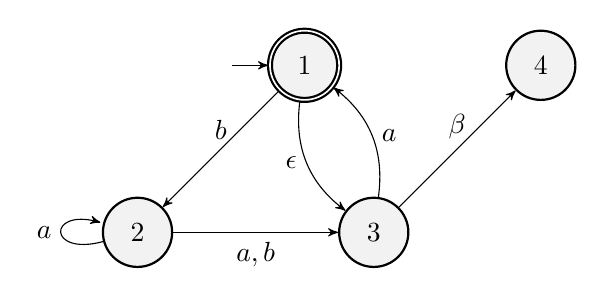
\begin{tikzpicture}

        \node[state, initial, accepting] (1) {$1$};
\node[state, below left of=1] (2) {$2$};
\node[state, right of=2] (3) {$3$};
\node[state, right of=1] (4) {$4$};

\draw (1) edge[above] node{$b$} (2)
      (1) edge[below, bend right, left=0.3] node{$\epsilon$} (3)
      (2) edge[loop left] node{$a$} (2)
      (2) edge[below] node{$a, b$} (3)
      (3) edge[above, bend right, right=0.3] node{$a$} (1)
      (3) edge[above] node{$\beta$} (4);

        
        \end{tikzpicture}
    \end{figure}
\end{document}